\chapter{Introduction} % Main chapter title

\label{Chapter1} % For referencing the chapter elsewhere, use \ref{Chapter1} 

%----------------------------------------------------------------------------------------

% Define some commands to keep the formatting separated from the content 
%\newcommand{\keyword}[1]{\textbf{#1}}
%\newcommand{\tabhead}[1]{\textbf{#1}}
%\newcommand{\code}[1]{\texttt{#1}}
%\newcommand{\file}[1]{\texttt{\bfseries#1}}
%\newcommand{\option}[1]{\texttt{\itshape#1}}

%----------------------------------------------------------------------------------------

\section{Pollution}

Pollution is defined as the presence of a substance in the environment orchestrating harmful or poisonous effects. Pollution could be broadly classified into two categories, one exists in form of chemical substances and other in form of energy. Pollutants could be naturally occurring or artificially generated. Pollution is also classified into categories such as point source and non-point source.
\\
\\
\textbf{Point sources} : It is a single identifiable source of pollution in air, water, thermal, noise or light. 
\\
\\
\textbf{Non-point sources}: It results from many diffused sources, generally from land runoff, precipitation, atmospheric deposition, drainage, seepage, or hydrological modification (rainfall or snowmelt) where tracing the pollution back to a single source is difficult.

\section{History of Pollution}
Pollution started from prehistoric times when man created the first fire. According to a 1983 article in the journal Science, "soot" found on ceilings of prehistoric caves provides ample evidence of the high levels of pollution that was associated with inadequate ventilation of open fires. Metal forging appears to be a key turning point in the creation of significant air pollution levels outside the households. Core samples of glaciers in Greenland indicate increases in pollution associated with Greek, Roman and Chinese metal production, but at that time the pollution was comparatively small and could be handled by nature. 

\section{Types of Pollution}
The major forms of pollution are listed below along with particular contaminants relevant to each of them:

\subsection{Air Pollution}
It occurs when harmful substances including particulates and biological molecules are introduced into Earth's atmosphere. Common gaseous pollutants include carbon monoxide, sulphur dioxide, chlorofluorocarbons (CFCs) and nitrogen oxides that are produced as by-products in industry and motor vehicles. Ozone and smog are created as nitrogen oxides and hydrocarbons react to sunlight. Particulate matter, or fine dust is characterized by their micrometre size PM10 to PM1.
\begin{figure}[h]
\begin{center}
 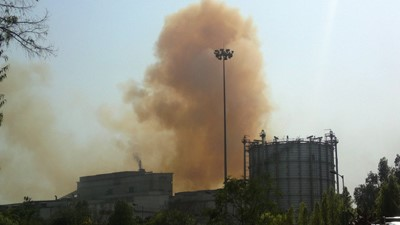
\includegraphics[width=80mm]{air.jpg}
 \caption{Air Pollution}
   \label{fig:Air Pollution}
\end{center}
\end{figure}

\subsection{Water Pollution}
It is the contamination of water bodies (e.g. lakes, rivers, oceans, aquifers and groundwater). It is caused by the discharge of wastewater from commercial and industrial waste (intentionally or through spills) into surface waters; discharges of untreated domestic sewage, and chemical contaminants, such as chlorine, from treated sewage; release of waste and contaminants into surface runoff flowing to surface waters (including urban runoff and agricultural runoff, which may contain chemical fertilizers and pesticides); waste disposal and leaching into groundwater; eutrophication and littering.

\begin{figure}[h]
 \centering
  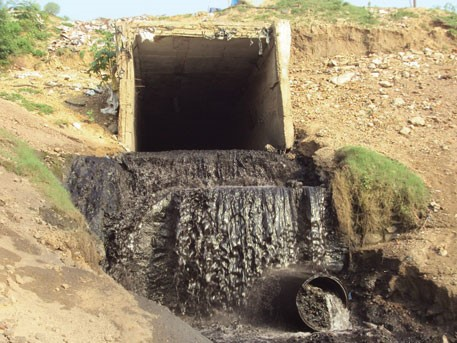
\includegraphics[width=80mm]{water.jpg}
  \caption{Water Pollution: Tata Steel discharge}
  \label{fig:Water Pollution: Tata Steel discharge}
\end{figure}

\subsection{Soil Pollution}
It is a part of land degradation is caused by the presence of XenoBionis (human-made) chemicals or other alteration in the natural soil environment. It is typically caused by industrial activity, agricultural chemicals, or improper disposal of waste, spill or underground leakage. Among the most significant soil contaminants are hydrocarbons, heavy metals, MTBE, herbicides, pesticides and chlorinated hydrocarbons.


\begin{figure}[h]
\centering
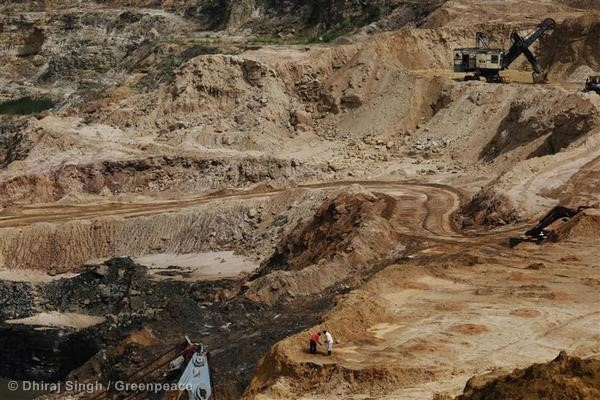
\includegraphics[width=0.5\textwidth]{./soil}\\[0.1in]
\label{Soil pollution: Durgapur coalmine}
 \caption{Soil Pollution Durgapur Coalmine}
 \label{soil pollution}
\end{figure}



\subsection{Noise Pollution}
Also known as noise disturbance is the disturbing or excessive noise that may harm the activity or balance of human or animal life. The source of most outdoor noise worldwide is mainly caused by machines and transportation systems, motor vehicles engines, aircraft, and trains.

%\begin{center}
%\begin{figure}
%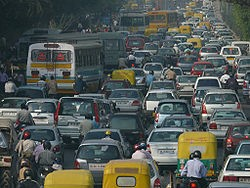
\includegraphics[width=0.6\textwidth]{./noise1}\\[0.1in]
 %\caption{noise pollution}
%\end{figure}
%\end{center}

\begin{figure}[h]
\centering
  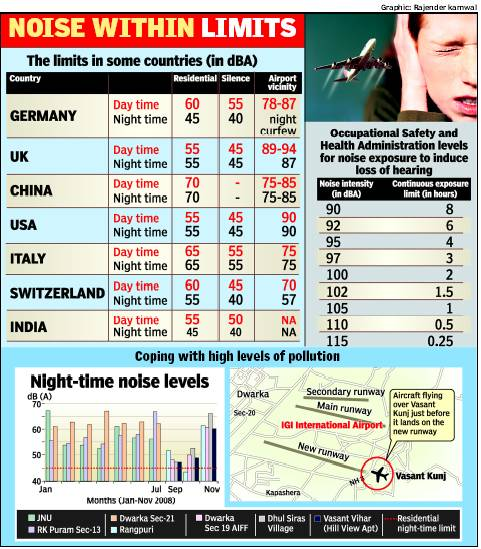
\includegraphics[width=80mm]{noise.jpg}
  \caption{Noise Pollution}
  \label{fig:Noise Pollution}
\end{figure}


\subsection{Radioactive Contamination}
It is resulting from 20th century activities in atomic physics, such as nuclear power generation and nuclear weapons research, manufacture and deployment. It is the deposition of, or presence of radioactive substances on surfaces or within solids, liquids or gases (including the human body), where their presence is unintended or undesirable. Such contamination presents a hazard because of the radioactive decay of the contaminants, which emit harmful ionising radiation such as alpha particles or beta particles, gamma rays or neutrons. The degree of hazard is determined by the concentration of the contaminants, the energy of the radiation being emitted, the type of radiation, and the proximity of the contamination to organs of the body.
%\begin{center}
%\begin{figure}
%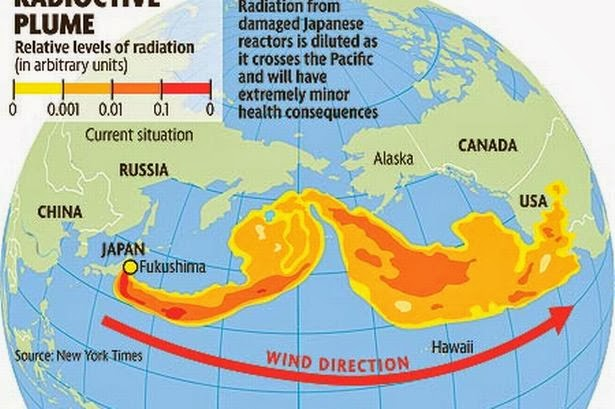
\includegraphics[width=0.60\textwidth]{./radiation}\\[0.1in] 
 %\caption{radioactive pollution}
%\end{figure}
%\end{center}

\begin{figure}[h]
\centering
  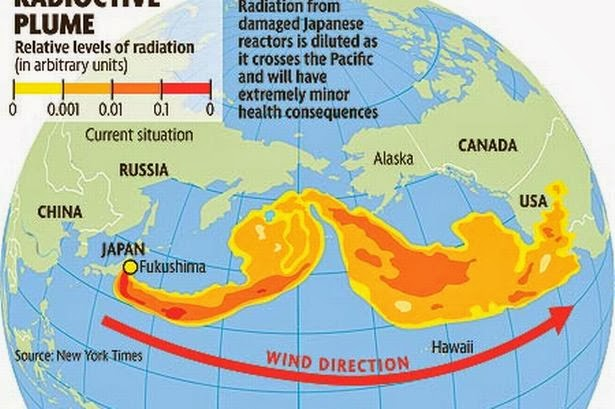
\includegraphics[width=70mm]{radiation.jpg}
  \caption{Radioactive Pollution}
  \label{fig:Radioactive Pollution}
\end{figure}




%%\subsection{Littering}
%%It consists of waste products that have been disposed improperly, without consent, at an inappropriate location.
%%\begin{figure}[h]
%%  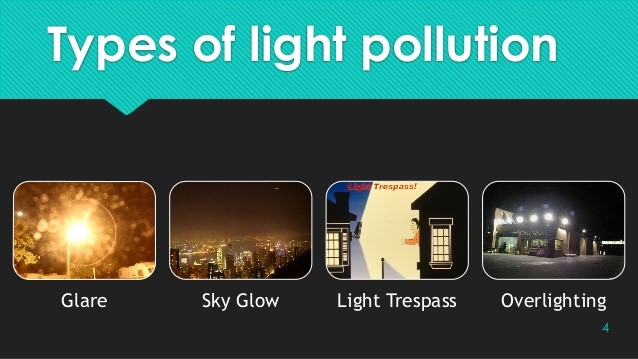
\includegraphics[width=\linewidth]{light_pollution.jpg}
%%  \caption{Air Pollution}
%%  \label{fig:Air Pollution}
%%\end{figure}

%\subsection{Thermal Pollution}
%It is the degradation of water quality by any process that changes ambient water temperature. A common cause of thermal pollution is the use of water as a coolant by power plants and industrial manufacturers. When water used as a coolant is returned to the natural environment at a higher temperature, the change in temperature decreases oxygen supply and affects ecosystem composition. Fish and other organisms adapted to particular temperature range can be killed by an abrupt change in water temperature (either a rapid increase or decrease) known as "thermal shock". Urban runoff—stormwater discharged to surface waters from roads and parking lots—can also be a source of elevated water temperatures.

%\begin{center}
%\begin{figure}
%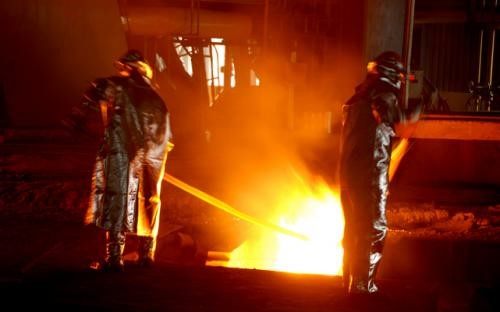
\includegraphics[width=0.60\textwidth]{./thermal}\\[0.1in]
 %\caption{Thermal pollution: SAIL Durgapur}
 %\label{Thermal pollution: SAIL Durgapur}
%\end{figure}
%\end{center}

%\begin{figure}[h]
 %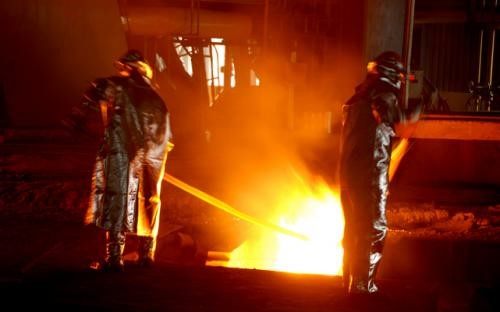
\includegraphics[width=\linewidth]{thermal.jpg}
  %\caption{thermal Pollution}
  %\label{fig:thermal Pollution}
%\end{figure}

%\subsection{Visual Pollution}
%It is an aesthetic issue and refers to the impacts of pollution that impair one's ability to enjoy a %vista or view. It disturbs the visual areas of people by creating harmful changes in the natural %environment. Pollution which can refer to the presence of overhead power lines, motorway billboards, %scarred landforms (as from strip mining), open storage of trash, municipal solid waste or space debris.

%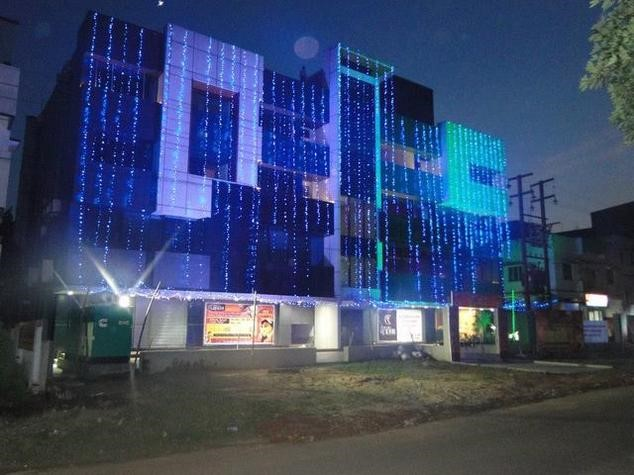
\includegraphics[width=1.0\textwidth]{./light}\\[0.1in]
%\begin{figure}[h]
 % 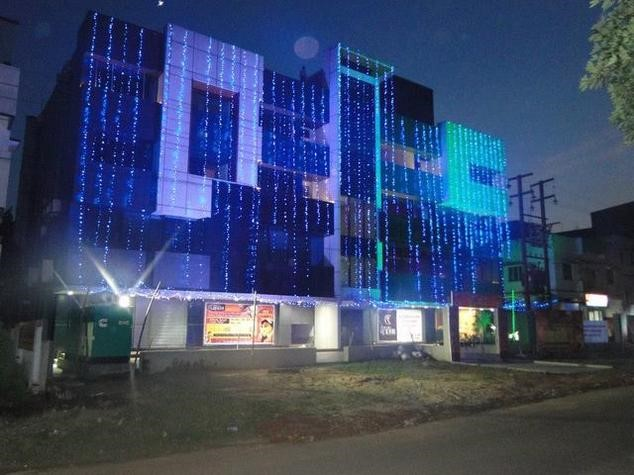
\includegraphics[width=\linewidth]{light.jpg}
  %\caption{light Pollution}
  %\label{fig:light Pollution}
%\end{figure}

%\subsection{Plastic Pollution}
%It involves the accumulation of plastic products in the environment that adversely affects wildlife, wildlife habitat, or humans. Plastics that act as pollutants are categorized into micro-, meso-, or macro debris, based on size.
%\begin{center}
%\begin{figure}
%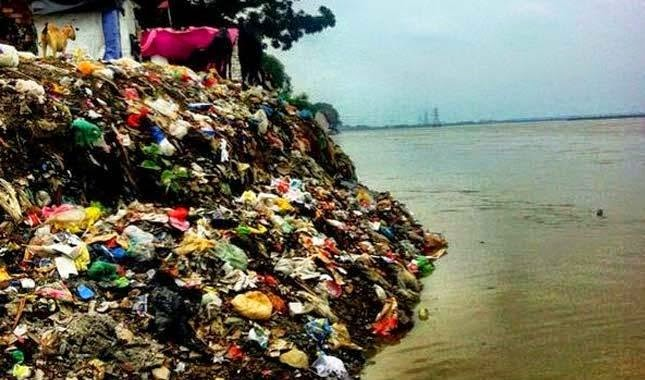
\includegraphics[width=0.70\textwidth]{./plastic}\\[0.1in]
 %\caption{Plastic Pollution}
%\end{figure}
%\end{center}

%\begin{figure}[h]
%\centering
 % 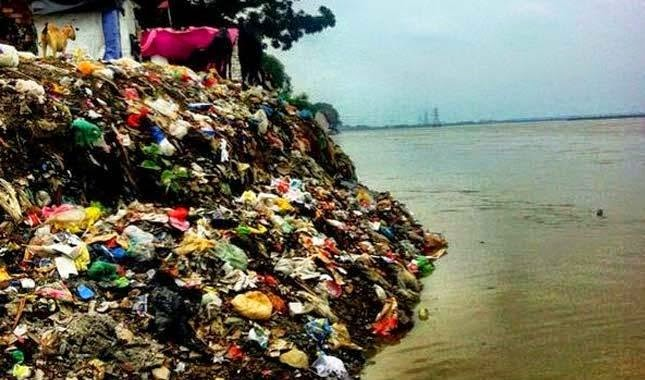
\includegraphics[width=100 mm]{plastic.jpg}
  %\caption{Plastic Pollution}
  %\label{fig:Plastic Pollution}
%\end{figure}

\section{Air Pollution}
Air pollution is by far the most harmful form of pollution in these times. Air pollution is caused by the harmful gases emitted by cars, buses, trucks, trains, and factories. Gases like sulphur dioxide, carbon mono oxide and nitrogen dioxide are very harmful to the environment causing a lot of damage to humans, animals and the atmosphere. Evidence of increasing air pollution can be anticipated by the galloping rates of lung cancer, asthma, allergies, and various breathing problems along with severe and irreparable damage to flora and fauna. Even the most natural phenomenon of migratory bird has been hampered due to the contaminated air around the world.

\subsection{Air Pollutants}
An air pollutant is a substance suspended in the air that have adverse effects on humans, animals and the ecosystem. The substance can be solid particles, liquid droplets, or gases. A pollutant can be of natural origin or artificially produced. Pollutants are classified as primary or secondary. Primary pollutants are usually produced from a process, such as ash from a volcanic eruption, carbon monoxide gas from motor vehicle exhaust, or the sulphur dioxide released from factories. Secondary pollutants are not emitted directly. Rather, they form in the air when primary pollutants react or interact with other elements or compound in nature. Ground level ozone is a prominent example of a secondary pollutant. Some pollutants may be both primary and secondary: they are both emitted directly and formed from other primary pollutants.
\\
\\
Substances emitted into the atmosphere by human activity includes:
\subsubsection{Nitrogen Dioxide}
Nature and Sources of the Pollutant: Nitrogen dioxide belongs to a family of highly reactive gas called Nitrogen Oxides ($NO_x$). These gases are formed when fuel is burned at high temperatures, and come principally from motor vehicle exhaust and stationary sources such as electric utilities and industrial boilers.
\\
\\
Health and Other effects: Nitrogen dioxide can irritate the lungs and lower resistance to the respiratory system of the human body causing infection such as influenza.
\\
\\
Ambient Level: LPA Inc.'s health-based national air quality standard for NO2 is 0.053 ppm

\subsubsection{Sulphur Dioxide}
Nature and Sources of the Pollutant: Sulphur dioxide belongs to the family of Sulphur dioxide gases ($SO_x$). These gases are formed when fuel containing Sulphur (mainly coal and oil) is burned, and during metal smelting and also in many other industrial processes.
\\
\\
Health and Other Effects: The major health concerns associated with exposure to high concentrations of $SO_2$ include effects on breathing, respiratory illness, alterations in pulmonary defences, and aggravation of existing cardiovascular disease. Together, $SO_X$ and $NO_X$ are the major precursors to acid rain, which is associated with the acidification of fresh water lakes and streams, accelerated corrosion of buildings and monuments, and reduced visibility. 
\\
\\
Ambient Level: EPA Inc.'s health-based national air quality standard for $SO_2$ is 0.03 ppm (measured on an annual average) and 0.14 ppm (measured over 24 hours).

\subsubsection{Carbon Monoxide}
Nature and Sources of the Pollutant: Carbon monoxide is a colourless and odourless poisonous gas formed when carbon in fuels is not burned completely. It is a by-product of motor vehicle exhaust, which contributes more than two-thirds of all CO emissions nationwide.
\\
\\
Health and Other Effects: Carbon monoxide enters the bloodstream and reduces oxygen delivery to the body's organs and tissues. The health threat from CO is most serious for those who suffer from cardiovascular disease. Elevated CO levels is associated with visual impairment, reduced work capacity, reduced manual dexterity, poor learning ability, and difficulty [measured over 8 hours] in performing complex task.
\\
\\
Ambient Level: EPA Inc.'s health based national air quality standard for CO is 9 parts per million (PPM).

\subsubsection{Carbon Dioxide}
Because of its role as a greenhouse gas it has been described as "the leading pollutant" and "the worst climate pollution". Against this, it is argued that carbon dioxide is a natural component of the atmosphere, essential for plant life and respired out by the human and animal respiratory system. This question of terminology has practical effects, for example as determining whether the U.S. Clean Air Act is deemed to regulate $CO_2$ emissions. $CO_2$ currently forms about 405 parts per million (ppm) of earth's atmosphere, compared to about 280 ppm in pre-industrial times, and billions of metric tons of $CO_2$ are emitted annually by burning of fossil fuels. $CO_2$ increase in earth's atmosphere has been accelerating.

\subsubsection{Particulate matter ($PM_{1O}$, $PM_{2.5}$ and $PM_1$)}
Nature and Sources of the Pollutants: Particulate matter is the term for solid or liquid particles found in the air. They originate from a variety of mobile and stationary sources (diesel trucks, wood stoves, power plants etc.).
Health and Other Effects: Major concerns for human health from exposure to particulate matter are- effects on breathing and respiratory systems, damage to lung tissue, cancer, and premature death. 
Ambient Level: EPA Inc.'s health-based national air quality standard for $PM_{10}$ is 50 micrograms per cubic meter (measured as an annual average).

\subsection{Types of Air Pollution}
\textbf{Outdoor Air Pollution}:
Smog is a type of large-scale outdoor pollution. It is caused by chemical reactions between pollutants derived from different sources, primarily automobile exhaust and industrial emissions. Cities are often centres of these types of activities, and many suffer from the effects of smog, especially during the warm months of the year.
\\
\\
\textbf{Indoor Air Pollution}:
Indoor air pollution is the presence of one or more contaminants indoors that carry a certain degree of human health risk. Indoor air issues may be traced to the beginning of civilization. Prehistoric records note the problem of smoke in caves. However, over the last three decades the public has become more aware of indoor air pollution. Various studies show that people spend 65 to 90 percent of their time indoors; 65 percent of that time is spent at home. Field studies of human exposure to air pollutants indicate that indoor air levels of many pollutants may be two to five times, and on occasion more than one hundred times, higher than outdoor levels.

\subsection{Effects of Air Pollution}
Air pollution can affect our health in many ways with both short-term and long-term effects. Different groups of individuals are affected by air pollution in different ways. Some individuals are much more sensitive to pollutants than are others. Young children and elderly people often suffer more from the effects of air pollution. People with health problems such as asthma, heart and lung disease may also suffer more when the air is polluted. The extent to which an individual is harmed by air pollution usually depends on the total exposure to the damaging chemicals, i.e., the duration of exposure and the concentration of the chemicals must be taken into account.
\\
\\
Examples of short-term effects include irritation to the eyes, nose and throat, and upper respiratory infections such as bronchitis and pneumonia. Other symptoms can include headaches, nausea, and allergic reactions. Short-term air pollution can aggravate the medical conditions of individuals with asthma and emphysema. In the great “Smog Disaster” in London in 1952, four thousand people died in a few days due to the high concentrations of pollution.
\\
\\
Long-term health effects can include chronic respiratory disease, lung cancer, heart disease, and even damage to the brain, nerves, liver, or kidneys. Continual exposure to air pollution affects the lungs of growing children and may aggravate or complicate medical conditions in the elderly. It is estimated that half a million people die prematurely every year in the United States as a result of smoking cigarettes.


\subsection{Increasing Mortality Rate due to Air Pollution}
The World Health Organization estimated in 2014 that every year air pollution causes the premature death of some 7 million people worldwide. India has the highest death rate due to air pollution. India also has more deaths from asthma than any other nation according to the World Health Organization. In December 2013 air pollution was estimated to kill 500,000 people in China each year. There is a positive correlation between pneumonia-related deaths and air pollution from motor vehicle emissions.
\\
\\
Annual premature European deaths caused by air pollution are estimated at 430,000. An important cause of these deaths is nitrogen dioxide and other nitrogen oxides ($NO_x$) emitted by road vehicles. Across the European Union, air pollution is estimated to reduce life expectancy by almost nine months. Causes of deaths include strokes, heart disease, COPD, lung cancer, and lung infections.
\\
\\
Urban outdoor air pollution is estimated to cause 1.3 million deaths worldwide per year. Children are particularly at risk due to the immaturity of their respiratory organ systems.
\begin{figure}[h]
\centering
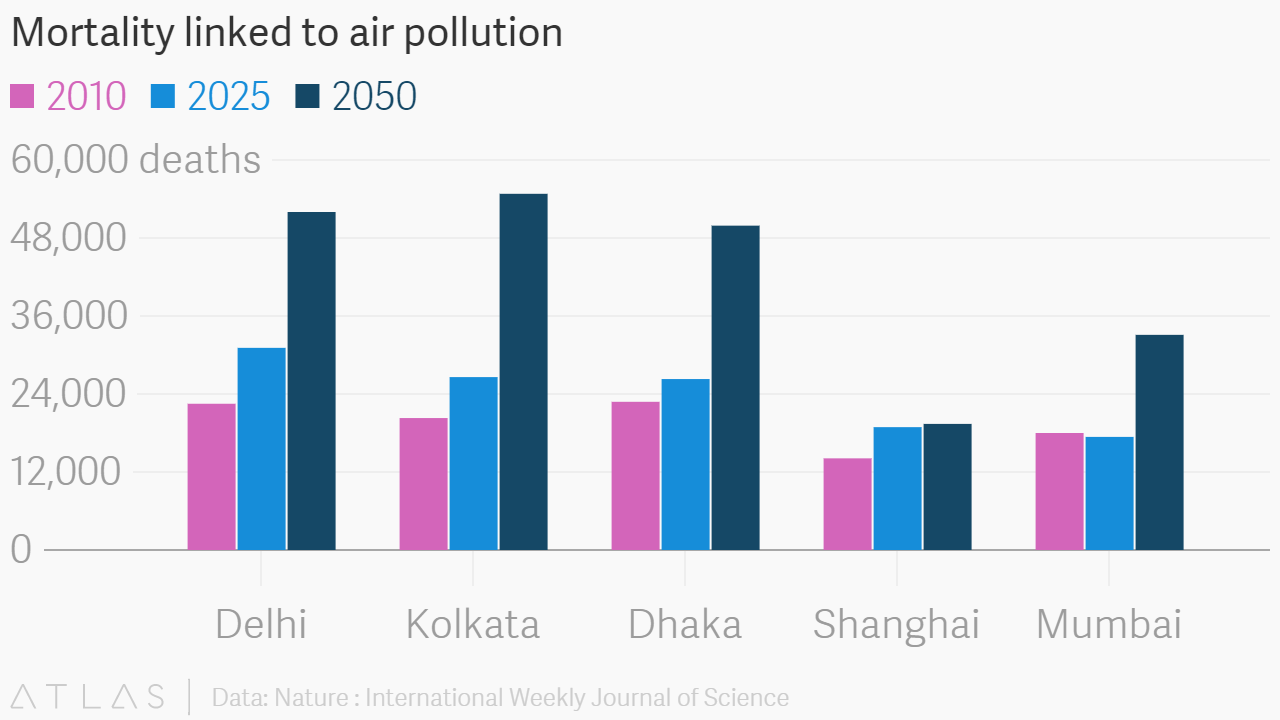
\includegraphics[width=0.8\textwidth]{./deadly}\\[0.1in]
\caption{Mortality linked to Air Pollution}
\label{fig: Mortality Linked to Air Pollution}
\end{figure}


\subsection{Major Air Pollution Incidents}

\subsubsection{Bhopal Gas Leak}
The world’s worst ever industrial accident happened on the night of December 2-3, 1984, when toxic gases leaked from the Union Carbide (now Dow Chemical) pesticide plant in Bhopal, India. The deadly fumes drifted into the sleeping city and people woke with burning eyes and lungs.
\\
\\
Thousands died within days. In the years after, pollutants seeping out of the plant site into groundwater have caused cancer, growth retardation and dizziness, say residents in Bhopal.

\subsubsection{Chernobyl Nuclear Accident}
The biggest radiation contamination ever happened on April 26, 1986 when the Chernobyl nuclear power plant’s core went into meltdown, killing 30 people and releasing 100 times more radiation than the atom bombs dropped on Japan. Even more radioactivity remains trapped within the plant.
\\
\\
From 1992 to 2002 in Belarus, Russia and Ukraine more than 4000 cases of thyroid cancer were diagnosed among children and adolescents, mainly due to contaminated milk. The 19-mile exclusion zone around the plant remains uninhabitable.

\subsubsection{Gulf of Mexico Oil Spill}
On April 20, 2010 the Deepwater Horizon offshore oil rig in the Gulf of Mexico exploded, killing 11 workers and leading to the worst oil spill and environmental catastrophe in US history.
\\
\\
A ruptured underwater pipe spewed almost 5 million barrels of oil into the Gulf over three months, threatening hundreds of miles of beaches, wetlands, and estuaries. Thousands of animals, including turtles, crabs, fish, and birds fell victim, and the local fishing and tourism industries suffered badly.

\subsection{Air Quality Index}
Air quality index (AQI) is a number used by government agencies  to communicate to the public how polluted the air currently is or how polluted it is forecast to become. As the AQI increases, an increasingly large percentage of the population is likely to experience increasingly severe adverse health effects. Different countries have their own air quality indices, corresponding to different national air quality standards.

\begin{figure}[h]
\centering
  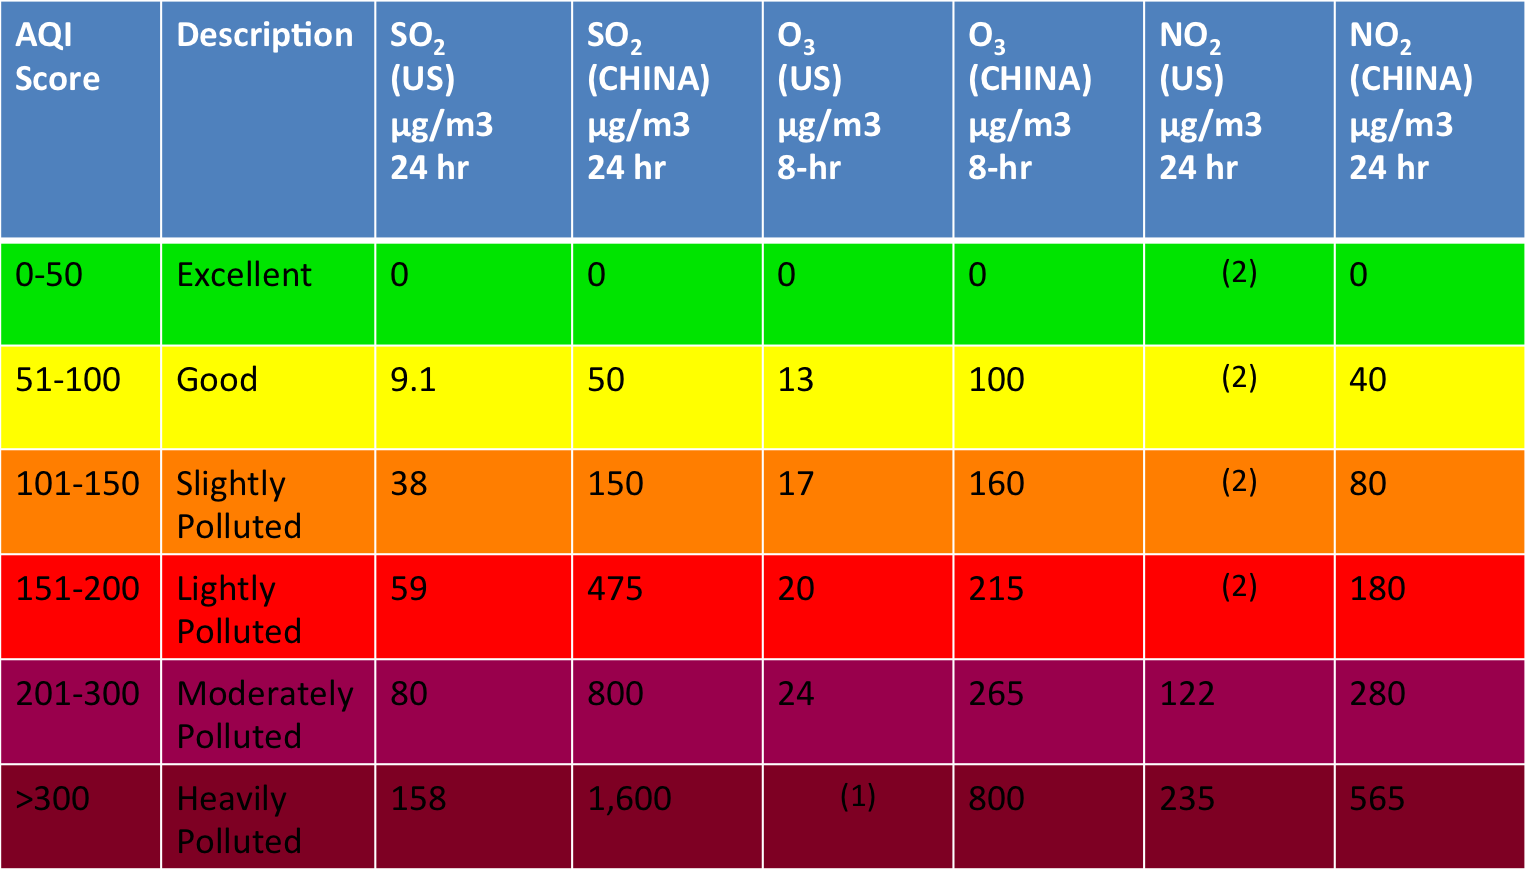
\includegraphics[width=0.8\textwidth]{./AQI}\\[0.1in]
  \caption{AQI categories and breakpoint concentrations with averaging times}
  \label{fig:AQI Category Breakpoint}
\end{figure}


The concept of an air quality Index (AQI) that transforms weighted values of individual air pollution related parameters (e.g. $S0_2$, CO, visibility, etc.) into a single number or set of numbers is widely used for air quality communication and decision making in many countries. Thus, An AQI is defined as an overall scheme that transforms weighted values of individual air pollution related parameters ($S0_2$. CO, visibility, etc.) into a single number or set of numbers.
%\begin{figure}[h]
 % 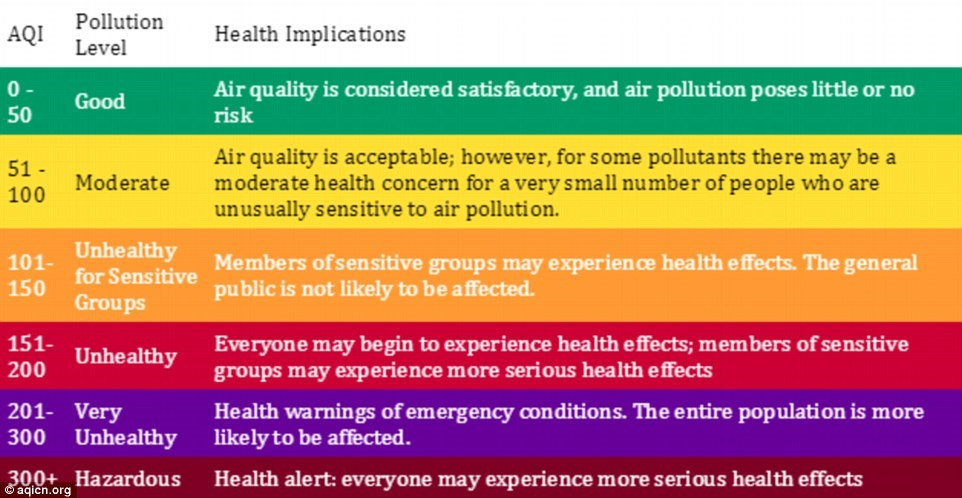
\includegraphics[width=\linewidth]{aqi2.jpg}
  %\caption{AQI levels}
  %\label{fig:AQI levels}
%\end{figure}

\section{Indoor pollution and Outdoor pollution comparison}

\textbf{Why is indoor air pollution more hazardous than outdoor air pollution?}
\\
\\
According to the EPA, our indoor environment is two to five times more toxic than our outdoor environment, and in some cases, the air measurements indoors have been found to be 100 times more polluted.
\\
\\
The International Agency for Research on Cancer and the World Health Organization have concluded that 80\% of all cancers are attributed to environmental rather than genetic factors, including exposure to carcinogenic chemicals, many of which are found in household cleaning products.
\\
\\
The World Health Organization (WHO) agrees, reporting that almost 3\% of the global burden of disease is due to indoor air pollution. We spend as much as 90\% of our lives indoors nowadays and researchers are investigating our exposure to indoor pollutants as contributing causes to rising incidence of autism, allergies and toxin load.
\\
\\
\textbf{Why do we need to measure air pollution?}
\\
\\
According to a report published earlier this year by the World Health Organisation, air pollution now kills approximately seven million people annually, worldwide. This accounts for as much as one in eight deaths, and is by far the single biggest environmental health risk.
\\
\\
In order to counteract this alarming statistic and take action to clean up air , it’s important to first understand where the pollution is most concentrated, how it occurs, what elements are involved and how we can neutralise them. In order to do this, comprehensive air monitoring must be undertaken on a national and international scale.
\\
\\
Among other pollutants, air monitors assess the amounts of carbon dioxide ($CO_2$), carbon monoxide (CO), nitrogen oxides ($NO_x$), ozone ($O_3$) and particulate matter 2.5 ($PM_2.5$). This allows us to see where and why pollution occurs, so that we can not only actively avoid overly contaminated areas in our daily routines but also try to implement measures to curb such pollution.

\begin{figure}[h]
\centering
  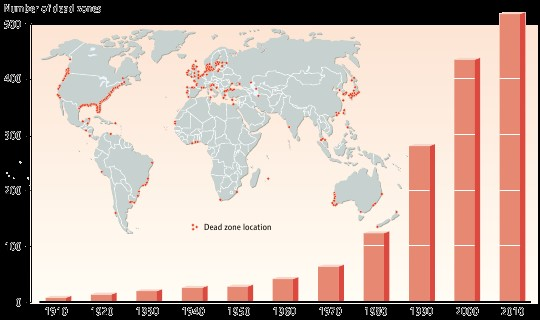
\includegraphics[width=100mm]{deadzone.jpg}
  \caption{AQI levels}
  \label{fig:AQI levels}
\end{figure}


\section{Site Survey}

\subsection{Present Scenario of Air Pollution}
Greenpeace analysed NASAs satellite data on particulate matter from 2003 to 2015 in India and China, and found that pollution levels in Chino peaked in 2011 and then started to gradually reduce. India, however, saw a spike over the past decade, the last year being the worst on record. The study looked at the aerosol optical depth (A0D), which is h the amount of fine solid particles and liquid droplets in air. The levels in India have increased over the years with north India being the most polluted part of the country. The biggest jump was seen in West Bengal, Bihar, Uttar Pradesh and the National capital Region. The report said that the AOD levels in Indian cities Patna, Kolkata, Delhi, Gorakhpur, Kanpur and Varanasi all went up from 2005 to 2015.
\\
\\
 There are large numbers of industries within West Bengal which are emitting harmful gases into the atmosphere and as a matter of fact, this emission is leading to tremendous amount of air pollution in major cities like Kolkata, Asansol, Durgapur and Raniganj. The extent of this pollution is so high, as to raise some serious environmental concerns. Presence of a large number of industries in Durgapur is the single biggest reason for the high level of pollution in this industrial industrial town and the biggest hurdle in the growth of this steel city and the only fact of concern for a healthy living.

\begin{figure}[h]
\centering
  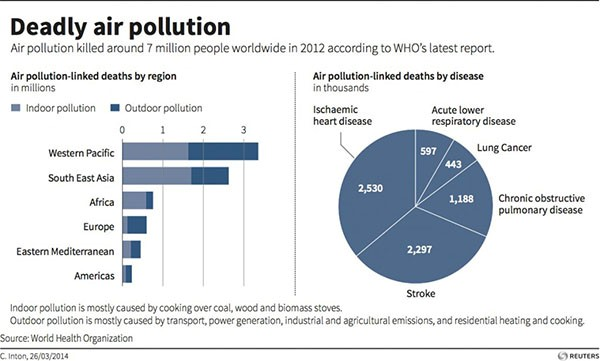
\includegraphics[width=100mm]{site_survey1.jpg}
  \caption{AQI levels}
  \label{fig:AQI levels}
\end{figure}

\begin{figure}[h]
\centering
  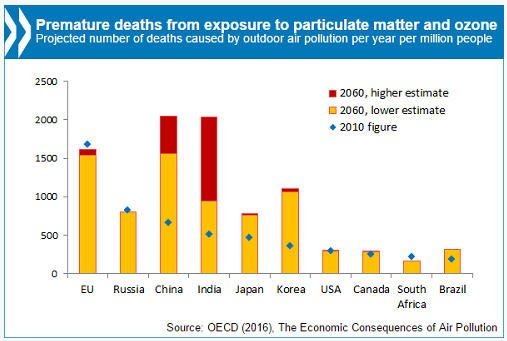
\includegraphics[width=100mm]{site_survey2.jpg}
  \caption{AQI levels}
  \label{fig:AQI levels}
\end{figure}

\subsection{Status of Air Pollution in Durgapur}
With pollution level increasing dangerously in the industrial belts of Haldia and Asansol, the union ministry of environment and forest had imposed a ban in 2010 declaring that no further industries could be set up in these industrial belts, the areas were classified as critically polluted zones. The centre as shortlisted Durgapur as the stage 2 of the smart city mission and the local civic body arranged a public hearing in this connection. The Durgapur Projects Limited (DPL), a state owned power utility, was asked to suspend generation as it continues to release Suspended Particulate Matter (SPM) in the ambient air. In December 2002 the WBPCB had introduced states first ambient air quality monitoring station in Durgapur, which however failed after a couple of years.
\\
\\
\textbf{NEWS FEED:}
\\
\\
\begin{enumerate}
	\item On 12th June 2015 Durgapur steel plant was hit by another mishap.
	\item On August 24, the West Bengal Pollution control board registered a police complaint against Durgapur Projects Limited (DPL), a state government undertaking, for violating pollution norms.
	\item Durgapur News Services, 26 December 2014: Recent revelation of the fact that pollution linked cancer patients on rise in Asansol-Durgapur.
\end{enumerate}

\subsection{Major Industries and pollutants emitted by them}

\begin{center}
 \begin{tabular}{| c |  p{4cm} | p{4cm} | p{4cm}| } 
 \hline
 Sl. & NAME & PRODUCT & POLLUTANTS \\ [0.5ex] 
 \hline\hline
 1 & Durgapur Steel Plant (D.S.P.) & P.R. TNIT Bars \& Rods, Angles, Channels, Wheel \& Axle & $S0_2$, $NO_x$, $CO_3$, Pb, Ni, As, Cd, Cr, ZnSe, Hg, PM \\ 
 \hline
 2 & Durgapur Thermal Power Station(D.V.C.) & P.R. Power Generation & $S0_2$, $NO_x$, Ni, As, Cr, Hg, Acid gases $S0_2$, $NO_x$, Hg, Acid gases \\
 \hline
 3 & The Durgapur Projects Ltd(D.P.L.)  & P.R. Power, Coke, Industrial Gas, Domestic Power, Industrial Power & $S0_2$, $NO_x$, Ni, As, Cr, Hg, Acid gases \\
 \hline
 4 & NTPC-SAIL Power CO Ltd & P.R. Power Generation \& Distribution & $S0_2$, $NO_x$, Ni, As, Cr, Hg, Acid gases \\
 \hline
 5 & Alloy Steel Plant & P.R. Stainless Steel, Billets etc. & Smoke, Fume, CO, Organic 
gases, PM, Organic matter \\
 \hline
 6 & Bharat Petroleum Corp. Ltd  & P.R. Petroleum Products \& Lubricants & $CO_2$, CO, methanol, soot, benzene, acid rains \\
 \hline
 7 & Birla Corporation Ltd  & P.R. Portland Slag Cement & $S0_2$, $NO_x$, CO, $CO_2$ \\
\hline
 8 & Durgapur Cements Works  & Cements Works & $S0_2$, $NO_x$, CO, $CO_2$ \\ 
\hline
 9 & Durgapur Chemicals Ltd.  & P.R. Caustic Soda, Benzene, Bleaching Pow-der, Sodium Chlorophenate, Hydrogen Gas, etc. & $S0_2$, $NO_x$, Benzene, Organic gases, Cl etc. \\
\hline
 10 & Graphite India Ltd  &Products of Graphite & PM, hydrocarbons, organic matter etc. \\  [1ex] 
 \hline
\end{tabular}
\end{center}